
\section{Transmon interactions}

An isolated transmon offers no mean of control and readout, so it is completely useless.
We have to add components for readout, drive (control of the qubit state) and flux (control of the qubit frequency).

For a single qubit, we can expect a scheme like the one represented in \cref{fig:scheme-basic_interaction}.

\begin{figure}[ht]
    \centering
    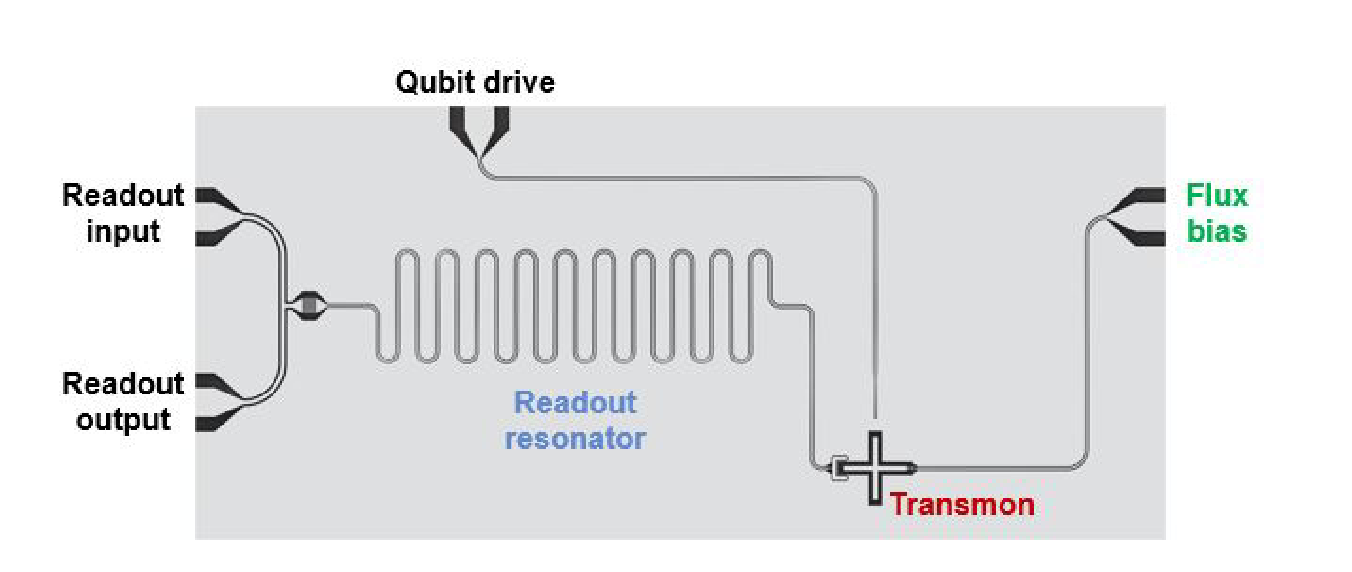
\includegraphics[width=0.8\textwidth]{Theory/figures/scheme_basic_interactions.png}
    \caption{Basic scheme for the complete control of a single flux-tunable transmon.}
    \label{fig:scheme-basic_interaction}
\end{figure}

In \cref{fig:scheme-basic_interaction} we can see all the standard lines present in a single qubit system:

\begin{description}
    \item[Readout input:] a line where a signal can be send to probe a resonator that is coupled to the qubit and, because of this, dependent on its state;
    \item[Readout output (feedback):] a line where the sent readout signal gets acquired, after the resonator interaction. This signal can be the input {\it reflected signal} (as in the scheme presented) or, in some configurations, the {\it transmitted signal}
    \item[Drive:] a line coupled to the qubit, that we can use to change the qubit state itself;
    \item[Flux:] a line that contains an inductor, so that a DC current passing through it can generate a magnetic field to change the qubit frequency.
\end{description}

An illustration, in circuit form, of the system is presented in \cref{fig:circuit-basic_interaction}.

\begin{figure}[ht]
    \centering
    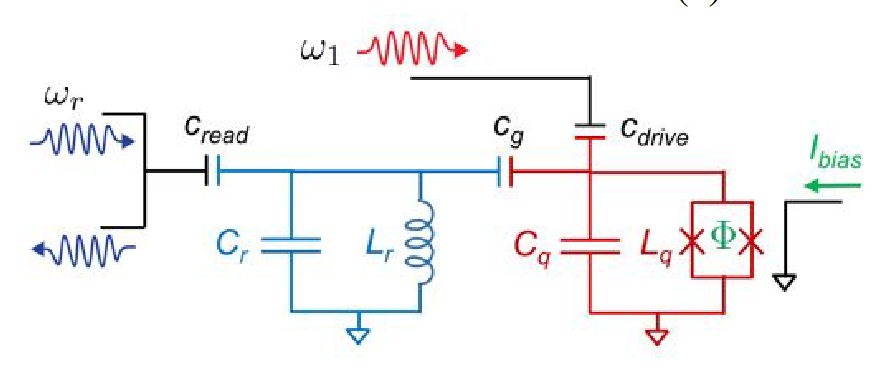
\includegraphics[width=0.8\textwidth]{Theory/figures/scheme_basic_interactions2.png}
    \caption{Basic circuit scheme for the complete control of a single flux-tunable transmon.}
    \label{fig:circuit-basic_interaction}
\end{figure}

To study the system we can start writing the Hamiltonian of the resonator-qubit system.
We can express the diagonalized qubit Hamiltonian, non limited to the first two states, as:
\begin{equation}
    \hat H_T = \sum_j \hbar \omega_j \ket j \bra j
\end{equation}
where $\omega_j$ is the eigenvalue associated with the $\ket j$ eigenstate.

The resonator Hamiltonian can be written in the standard harmonic oscillator form:
\begin{equation}
    \hat H_R = \hbar \omega_r \hat a^\dagger \hat a
\end{equation}

The total Hamiltonian of the system will add one more term:
\begin{equation}
    \hat H = \hat H_T + \hat H_R + \hat H_I
\end{equation}

The interaction term can be written as:
\begin{equation}
    \hat H_I = 2e \frac{C_g}{C_g+C_q}\hat V_r \hat n= 2e \frac{C_g}{C_g+C_q}V_{rms} (\hat a + \hat a ^ \dagger) \hat n
\end{equation}
where $\hat V_r$ is the resonator voltage operator and $V_{rms}=\sqrt{\hbar \omega/2C_r}$.\\
If we write the qubit charge operator in terms of the transmon eigenstates, define the coupling $g_j=2e\frac{C_g}{C_g+C_q} V_{rms} \bra{j-1} \hat n \ket{j}$ and simplify the equation considering only the relevant terms:
\begin{equation}\label{eq:jaynes-cummings-generalized}
    \hat H = \sum_j \hbar \omega_j \ket j \bra j + \hbar \omega_r \hat a^\dagger \hat a + \sum_j g_j (\ket{j-1} \bra{j}\hat a^\dagger  + \ket j \bra{j-1} \hat a)
\end{equation}
this equation is usually called \textit{Jaynes-Cummings Hamiltonian}.

To understand the simplification we can write the generalized Jaynes-Cumming Hamiltonian as:
\begin{equation}
    \hat H = \omega_r(\hat a ^ \dagger \hat a) - \frac{1}{2}\omega_1\sigma_z - g(\hat a ^ \dagger + \hat a)(\sigma_-+\sigma_+)
\end{equation}
where $\sigma_z$  is the Z Pauli matrix and the $\sigma_\pm$ are the transmon ladder operators.\\
This representation does not add anything to the previous one, but it could maybe be a bit more easy to understand when we focus on the interacting Hamiltonian:
\begin{equation}
    \hat H_{I} = \hat a ^ \dagger \sigma_- + \hat a \sigma_+ + \hat a ^ \dagger \sigma_+ + \hat a \sigma_-
\end{equation}
The first term describes a qubit decay while creating a new photon in the resonator and so on.\\
Now it's easy to identify that, of those 4 terms, only 2 conserve the energy and are much less likely to occur.
Actually, using the \textit{Rotating Wave Approximation} (RWA), we can remove these terms, reaching again the form of \cref{eq:jaynes-cummings-generalized}.

In the dispersive regime ($\Delta = \abs{\omega_j - \omega_r}\gg g_j$) we can define the \textit{dispersive shift} $\chi = g_1^2/\abs{\omega_1-\omega_r}$ and, considering only $\ket 0$ and $\ket 1$ as the first two transmon states, write:
\begin{equation}
    \hat H = \hbar (\omega_r - \chi \ket 1 \bra 1 + \chi \ket 0 \bra 0 ) \hat a ^ \dagger \hat a + \frac{\hbar}{2}(\omega_1 + \chi) (\ket 0 \bra 0 - \ket 1 \bra 1)
\end{equation}
or better:
\begin{equation}\label{eq:readout_equation}
    \hat H = (\omega_r - \chi \sigma_z) \hat a ^\dagger \hat a - \frac{1}{2}\omega_q\sigma_z
\end{equation}
where $sigma_z$ is the Pauli matrix and $\omega_q =\omega_1$.

This is the relation exploited in the standard transmon readout scheme.

